
\chapter{Integrali}
\section{I Problemi del Calcolo Integrale}
L'integrale nasce per risolvere due problemi:
\begin{enumerate}
    \item Area dei rettangoloidi.
    \begin{center}
    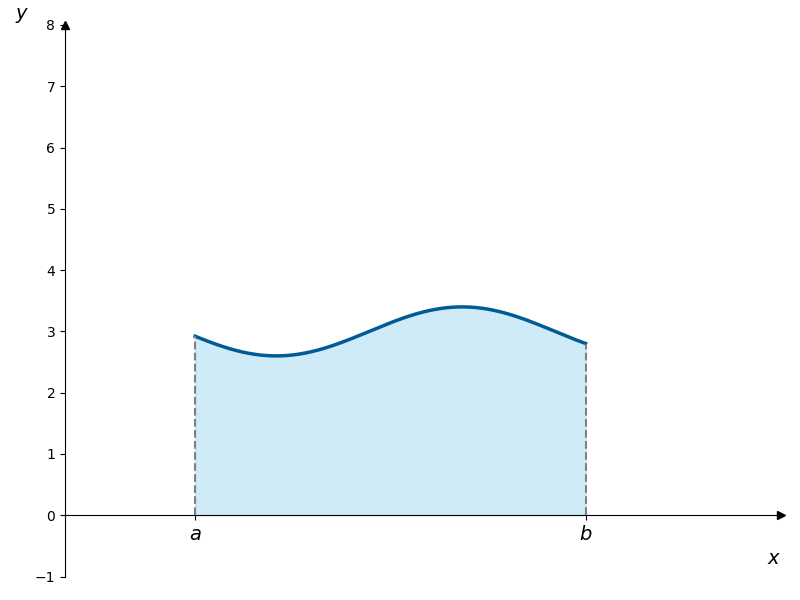
\includegraphics[width=0.7\textwidth]{img/rettangoloide.png}
    \end{center}
    \item Assegnata $f$:
    \[
    \exists F : F' = f
    \]
\end{enumerate}

\section{Integrale Definito}
Archimede ha calcolato l'area del settore parabolico "imprigionandola" tra due approssimazioni:
\begin{itemize}
    \item \textbf{Sottostima}: Ha sommato le aree di rettangoli inscritti (dentro la curva), ottenendo un valore inferiore a quello reale.
    \item \textbf{Sovrastima}: Ha sommato le aree di rettangoli circoscritti (fuori dalla curva), ottenendo un valore superiore.
\end{itemize}

\defn{Somma integrale superiore ed inferiore}{
    Sia $f: [a,b]\to \mathbb{R}$ limitata. Si definisce partizione di $[a,b]$ l'insieme:
    \[ P = \{ x_{0}=a, x_1 , x_2 , \dots , x_n = b : x_0 =a < x_1 < x_2 < \dots < x_n = b \} \]
    Consideriamo un generico intervallo $[x_k , x_{k+1}]$.
    Chiamiamo $m_k = \inf_{[x_k , x_{k+1}]} f(x)$ e $M_k = \sup_{[x_k , x_{k+1}]} f(x)$ che sono finiti essendo $f$ limitata.
    
    Si definisce \textbf{somma integrale inferiore} di $f$, relativa a $P$, la seguente:
    \[ s(P,f) = \sum_{k=0}^{n-1} m_k \cdot (x_{k+1} - x_k )= \sum_{k=1}^{n} m_k (x_k - x_{k-1}) \]
    Si definisce \textbf{somma integrale superiore} di $f$, relativa a $P$, la seguente:
    \[ S(P,f) = \sum_{k=0}^{n-1} M_k \cdot (x_{k+1} - x_k )= \sum_{k=1}^{n} M_k (x_k - x_{k-1}) \]
    Ovviamente $s(P,f)\leq S(P,f)$. Devo dimostrare $s \nearrow$ e $S \searrow$.
}

    \begin{center}
    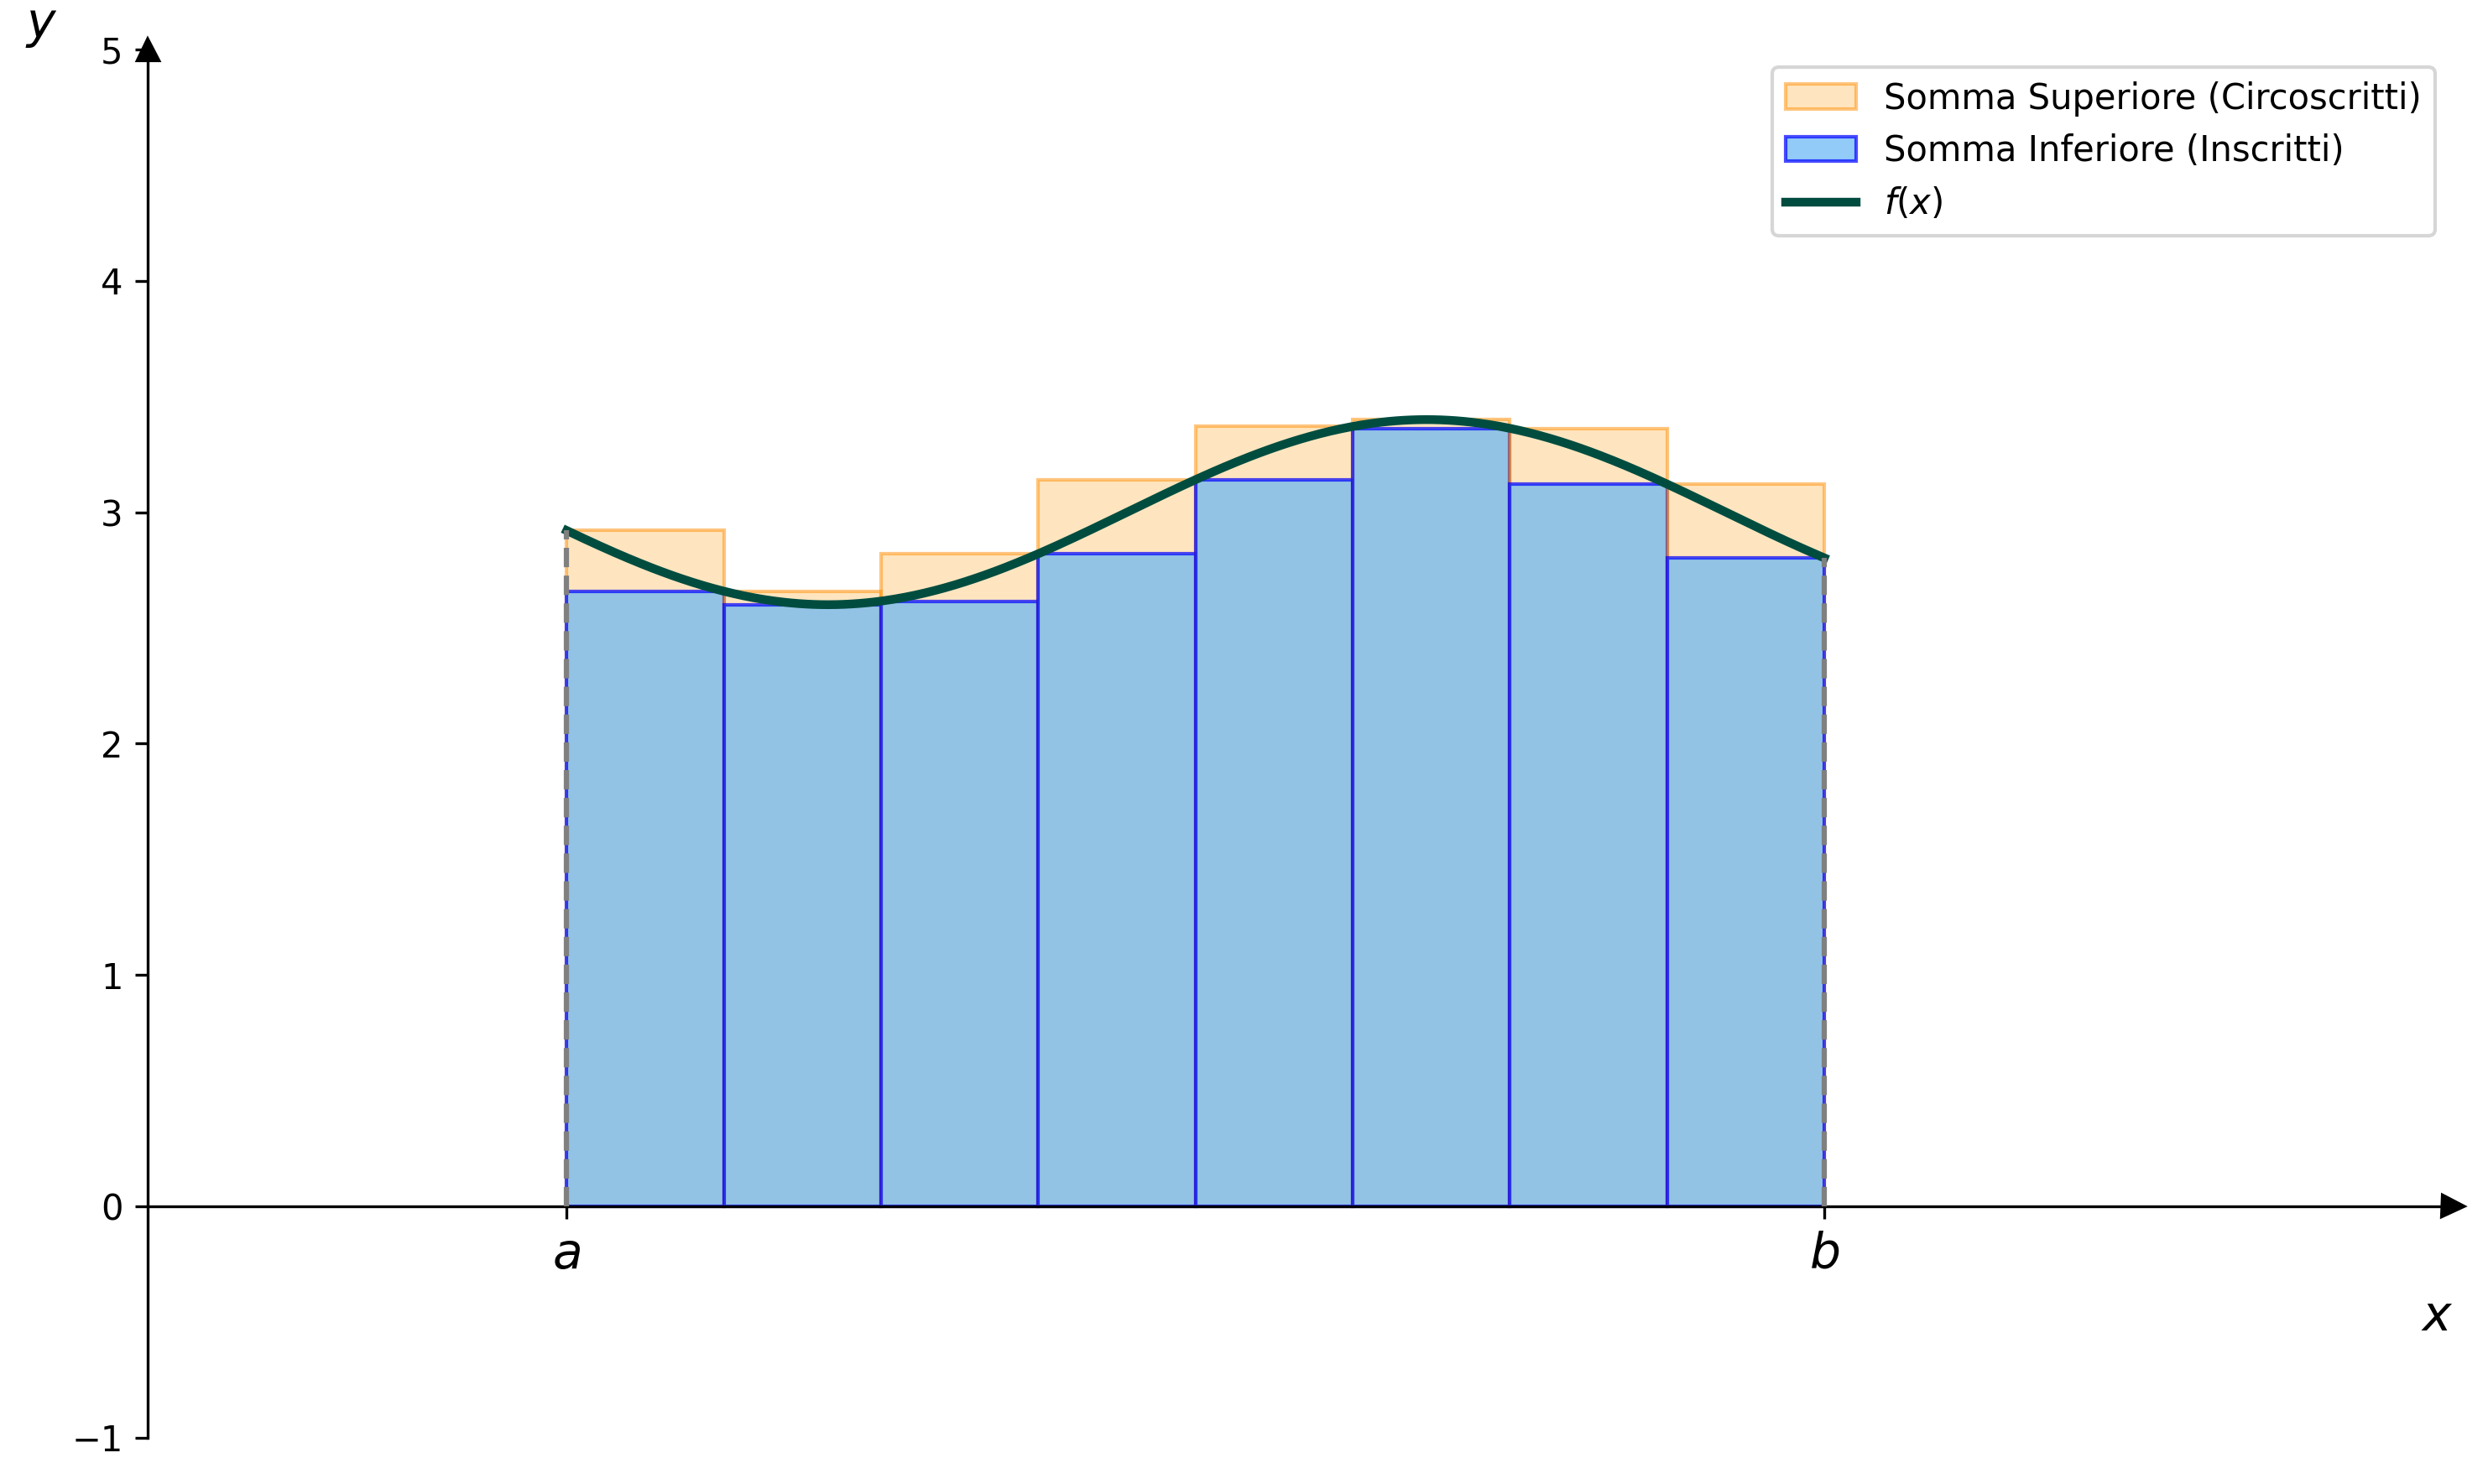
\includegraphics[width=0.8\textwidth]{img/stima_rettangoloide.png}
    \end{center}

\lem{}{
    Se $P \subseteq \overline{P}$ sono due partizioni di $[a,b]$ allora se $f: [a,b] \to \mathbb{R}$ è limitata, risulta che:
    \begin{align*}
    & s(P,f)\leq s(\overline{P},f)\\
    & S(P,f)\geq S(\overline{P},f)
    \end{align*}
}

\pf{
    Sia $P$ fissa, $P = \{ x_{0}=a , x_{1},x_{2},\dots, x_{n}=b \}$.

    Sia $\overline{P}= P \cup \{ z \}$.
    
    \begin{center}
    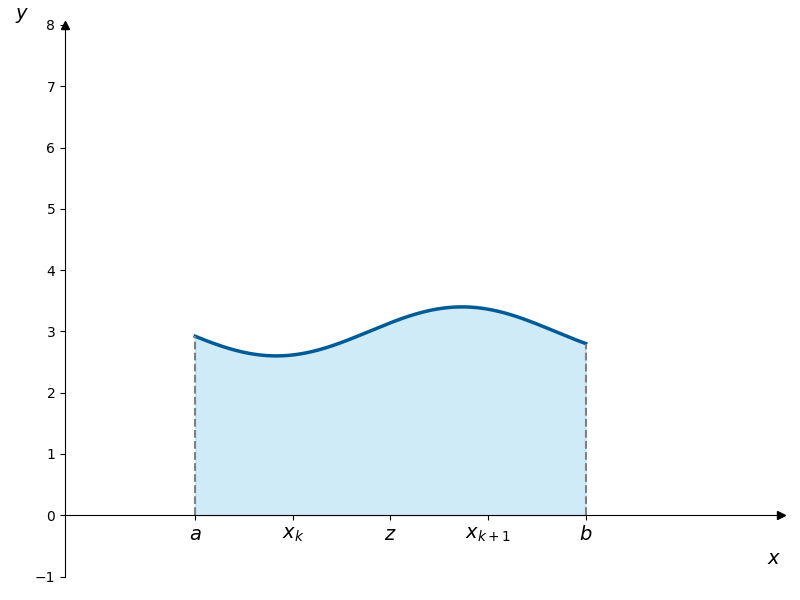
\includegraphics[width=0.8\textwidth]{img/rettangoloide_z.png}
    \end{center}


    \begin{align*} 
    & s(P,f)=m_{0}(x_{1}-a)+\dots+ \textcolor{orange}{m_{k}(x_{k+1}-x_{k})} +\dots+m_{n-1}(b-x_{n-1}) \\ 
    & s(\overline{P},f)= m_{0}(x_{1}-a)+\dots+\textcolor{orange}{m'_{k}(z -x_{k})+m''_{k}(x_{k+1}-z)}+\dots+m_{n-1}(b-x_{n-1}) 
    \end{align*}
    Dove:
    \[ m'_{k}=\inf_{[x_{k},z]}f\geq m_{k} \quad \text{e} \quad m''_{k}=\inf_{[z,x_{k+1}]}f\geq m_{k} \]
    Poiché $m'_k \ge m_k$ e $m''_k \ge m_k$ (l'inf su un insieme più piccolo è $\ge$ dell'inf sull'insieme grande), si ha:
    \begin{align*}
    &m'_{k}(z-x_{k})+m''_{k}(x_{k+1}-z)\geq m_{k}(z-x_{k}+x_{k+1}-z)\implies \\
    &m'_{k}(z-x_{k})+m''_{k}(x_{k+1}-z)\geq m_{k}(x_{k+1}-x_{k}) 
    \end{align*}
    Allora $s(P,f) \nearrow$. Allo stesso modo per $S(P,f)$.
}

\lem{Key-Lemma}{
    $\forall P, Q$ partizioni di $[a,b]$. Se $f:[a,b]\to \mathbb{R}$ è limitata, allora:
    \[ s(P,f)\leq S(Q,f) \]
        \begin{center}
    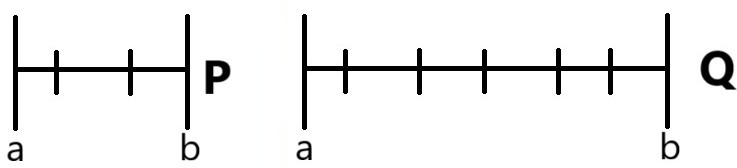
\includegraphics[width=0.8\textwidth]{img/key_lemma.jpg}
    \end{center}
}

\pf{
    Sia $R=P \cup Q$.
    \[ s(P,f)\le s(R,f)\leq S(R,f) \le S(Q,f) \]
}

\defn{Funzione integrabile secondo Riemann}{
    Definiamo:
    \[ A(f)=\{ S(P,f) , \quad P \text{ partizione} \} \]
    \[ B(f)=\{ s(P,f) , \quad P \text{ partizione} \} \]
    Allora $A(f)$ e $B(f)$ per il Key-Lemma sono separati, ovvero:
    \[ \inf A(f)=S(f)\geq \sup B(f)=s(f) \]
    Se sono contigui, ovvero $S(f)=s(f)=c$, allora diremo che $f$ è \textbf{integrabile} secondo Riemann.
    \[ c= \int_{\textcolor{magenta}{a}}^{\textcolor{magenta}{b}} \textcolor{blue}{f(x)} \, d\textcolor{orange}{x} \]
    e si chiama integrale definito.
    \[
    \begin{cases}
    \textcolor{magenta}{\text{Estremi di integrazione}}\\
    \textcolor{blue}{\text{Funzione integranda}}\\
    \textcolor{orange}{\text{Variabile d'integrazione}}
    \end{cases}
    \]
}

\subsection{Definizione con Limite}
Se voglio usare il limite:

\defn{Integrale definito con Limite}{
    Sia $P$ con passo $\frac{b-a}{n}$.
    \begin{align*}
    & s(P,f) \leq \frac{b-a}{n} \sum f(\overline{x}) \leq S(P,f) \quad \text{con } \overline{x}\in[x_{k},x_{k+1}]\\
    & \text{Le due quantità tendono rispettivamente a: } s(f) \text{ e } S(f)\\
    & \inf_{n}S(P_{n},f) = \sup_{n}s(P_{n},f)
    \end{align*}
}
    \begin{center}
    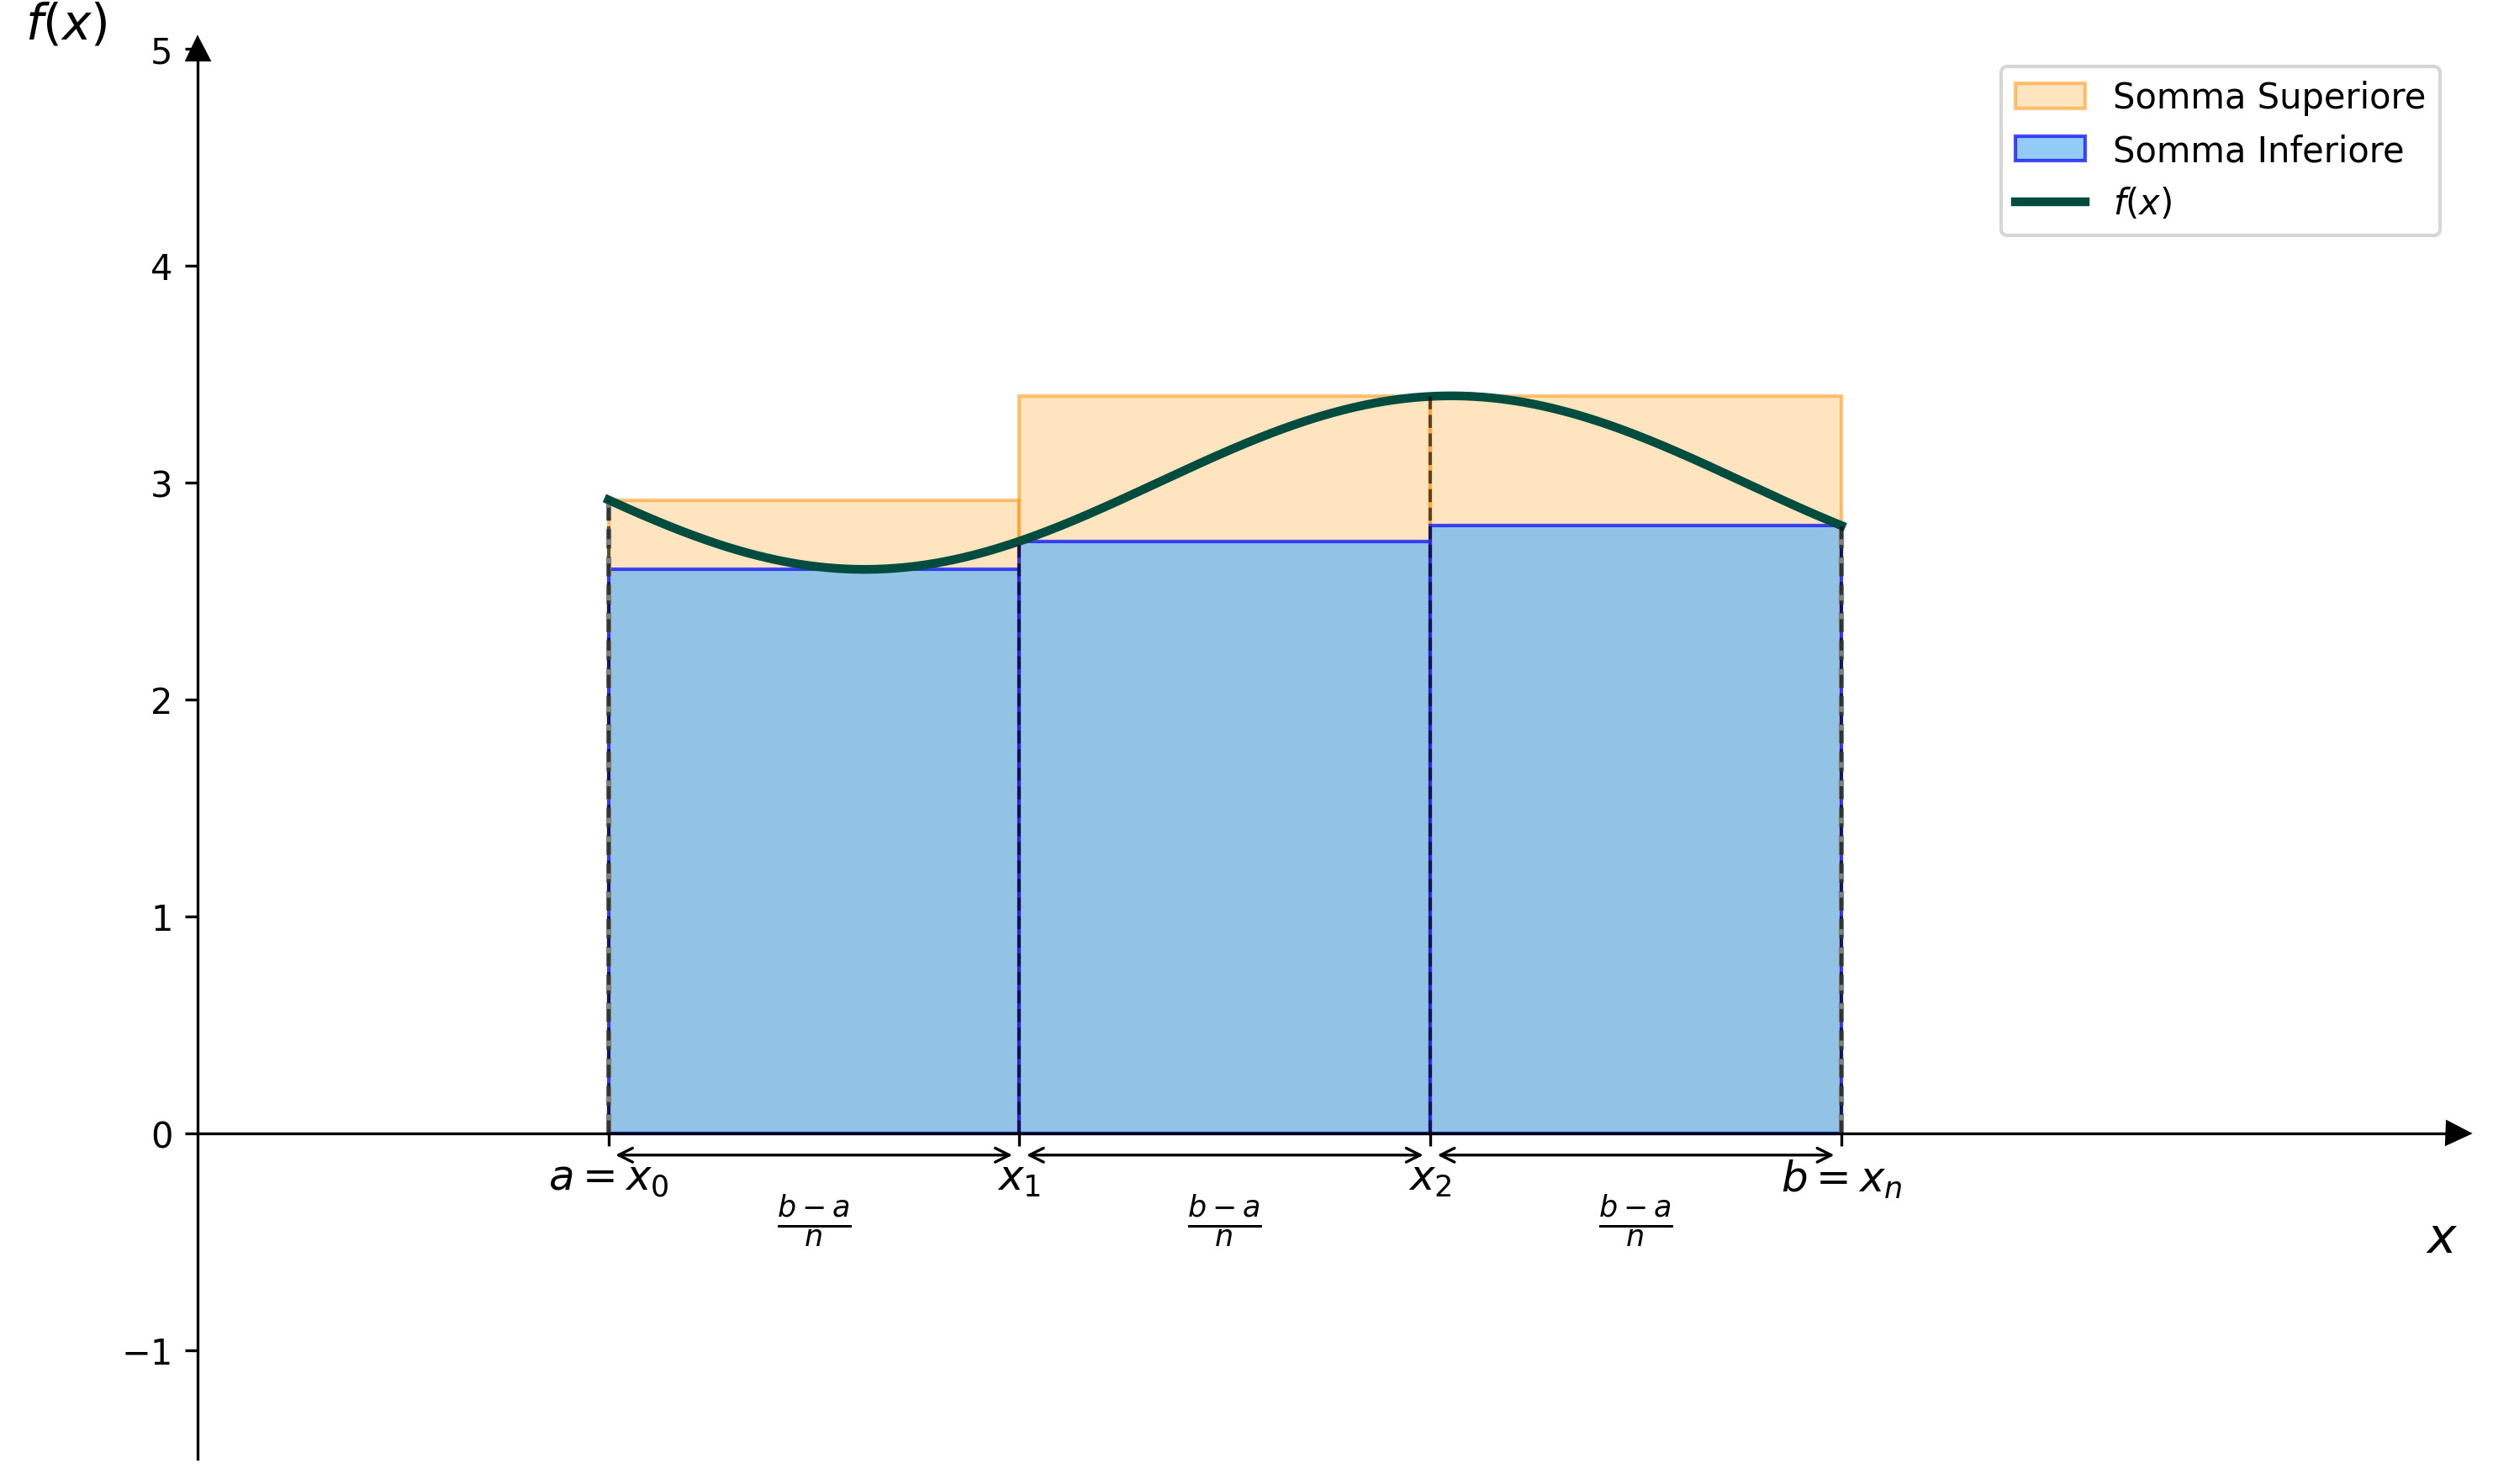
\includegraphics[width=0.8\textwidth]{img/stima_rettangoloide_n3.png}
    \end{center}

\ex{
    \textbf{Funzione di Dirichlet}: $f(x):[0,1]\to \{ 0,1 \}$
    \[
    f(x)=\begin{dcases}
    0 & x\in[0,1]\cap \mathbb{Q}\\
    1 & x\in[0,1]\setminus \mathbb{Q}
    \end{dcases}
    \]
    Considerando una partizione $P$:
    \begin{align*}
    &m_{k}= 0 \; \forall k \implies s(P,f)=0 \; \forall P\\
    &M_{k}= 1 \; \forall k \implies S(P,f)=\sum_{k=0}^{n} 1 \cdot (x_{k+1}-x_{k})=1  \; \forall P
    \end{align*}
}

\rmkb{
    Se $f\geq 0$ ed è integrabile in $[a,b]$ secondo Riemann, allora $\int_{a}^b f(x) \, dx$ geometricamente rappresenta l'area della porzione di piano compresa tra il grafico e l'asse $x$ che si chiama \textbf{Rettangoloide} relativo a $f$ di base $[a,b]$.
}

\rmkb{
    Se integro $f$ dispari in un intervallo simmetrico $[-a,a]$ allora:
    \[ \int^a_{-a} f(x) \, dx =0 \]
    Se $f$ è pari:
    \[ \int_{-a}^a f(x) \, dx =2\int_{0}^a f(x) \, dx \]
}

\subsection{Criterio di Integrabilità}
\prop{
    Sia $f$ limitata in $[a,b]$. $f$ è integrabile $\iff$ ($A(f),B(f)$ sono contigui) $\iff$
    $\forall \epsilon>0, \exists P \text{ partizione di } [a,b]:$
    \[ S(P,f)-s(P,f)<\epsilon \]
}

\subsection{Teorema Integrabilità delle funzioni continue}
\thm{Teorema Integrabilità delle funzioni continue}{
    Sia $f:[a,b]\to \mathbb{R}$ continua. Allora è integrabile secondo Riemann.
}

\pf{
    Per il Teorema di Heine-Cantor, $f$ è uniformemente continua.
    $\forall \epsilon>0, \exists \delta :$
    \[ |f(x')-f(x'')|<\epsilon \; \forall |x'-x''| < \delta \quad x', x'' \in [a,b] \]
    Sia $\epsilon$ fissato e sia $\delta$ il $\delta$ dell'uniforme continuità.
    Considero $P$ tale che $x_{k+1}-x_{k}$ è la stessa $\forall k$ e $x_{k+1}-x_{k}<\delta$.
    \[ S(P,f)-s(P,f)= \sum_{k=0}^{n} (M_{k}-m_{k})(x_{k+1}-x_{k})<\sum_{k=0}^{n} \epsilon(x_{k+1}-x_{k})=\epsilon(b-a) \]
}

\subsection{Teorema di Integrabilità delle Funzioni Monotone}
\thm{Teorema di Integrabilità delle Funzioni Monotone}{
    Sia $f$ monotona e $f:[a,b]\to \mathbb{R}$. Allora $f$ è integrabile secondo Riemann.
}

\pf{
    Immaginiamo $f$ crescente per fissare le idee. Si considera $P_{n}$ partizione di $n+1$ punti:
    \[ x_{k+1}-x_{k}=\frac{b-a}{n}\;\forall k = 0,\dots,n-1 \]
    \[ S(P_{n},f)= \sum_{k=0}^{n-1} M_{k}(x_{k+1}-x_{k})=\frac{b-a}{n} \sum_{k=0}^{n-1} M_{k} = \frac{b-a}{n}\sum_{k=0}^{n-1}f(x_{k+1}) \]
    \[ s(P_{n},f)=\frac{b-a}{n}\sum_{k=0}^{n-1} f(x_{k}) \]
    \begin{align*}
    & S(P_{n},f) - s(P_{n},f) = \frac{b-a}{n}\sum_{k=0}^{n-1} (f(x_{k+1})-f(x_{k})) \\
    & S(P_{n},f) - s(P_{n},f) = \frac{b-a}{n}(f(b)-f(a))
    \end{align*}
    Per il Criterio di Integrabilità, $f$ è integrabile.
}

\subsection{Proprietà degli integrali}
Siano $f,g: [a,b]\to \mathbb{R}$ integrabili. Allora:
\begin{enumerate}
    \item $f$ è integrabile in $[c,d]\subset [a,b]$.
    \item \textbf{Linearità}: $\int_{a}^b(\alpha f(x) +\beta g(x))\, dx = \alpha \int_{a}^b f(x) \, dx + \beta \int_{a}^b g(x) \, dx \quad \forall \alpha,\beta \in \mathbb{R}$.
    \item \textbf{Additività}: $\int_{a}^c f(x)\, dx + \int_{c}^b f(x) \, dx = \int_a^b f(x) \, dx \;\forall c \in ]a,b[$.
    \item Se $f(x)\leq g(x) \implies \int_{a}^b f(x) \, dx \leq \int_{a}^b g(x) \, dx$.
    \item Se $f(x)=k \quad \forall x \implies \int_{a}^b f(x) \, dx = k(b-a)$.
    \item Se $|f|$ è integrabile: $\left|\int_{a}^b f(x) \, dx\right|\leq \int_{a}^b |f(x)| \, dx$.
\end{enumerate}

\rmkb{
    Dalle proprietà 4 e 5, ottengo:
    \[ m (b-a) \leq \int_{a}^b f(x) \, dx \leq M (b-a) \]
    dove $m = \inf_{[a,b]} f$ e $M = \sup_{[a,b]} f$.
}

\subsection{Teorema della Media Integrale}
\prop{
    Sia $f: [a,b]\to \mathbb{R}$ continua. Allora $\exists c \in [a,b]:$
    \[ \int_{a}^b f(x) \, dx = f(c)(b-a) \]
}

\pf{
    Poniamo $y= \frac{\int_{a}^b f(x) \, dx}{b-a}$.
    Per le proprietà precedenti:
    \[ m\leq \frac{\int_{a}^b f(x) \, dx}{b-a} \leq M \]
    con $m=\min_{[a,b]}f$ e $M = \max_{[a,b]}f$ (poiché continua).
    Per il Teorema dei valori intermedi: $\exists c: y = f(c)$.
}

\subsection{Funzione Integrale}
\defn{Definizione}{
    Sia $f$ integrabile in $[a,b]$ e sia $x_{0}\in[a,b]$. Allora $\forall x \in [a,b]$ posso definire:
    \[ F(x)=\int_{x_{0}}^x  f(t) \, dt \]
    che si chiama \textbf{funzione integrale} relativa a $f$ di punto iniziale $x_{0}$.
}

\thm{Teorema Fondamentale del Calcolo Integrale}{
    Sia $f:[a,b]\to \mathbb{R}$ continua. Sia $x_{0}\in[a,b]$.
    Allora la funzione integrale $F(x)= \int_{x_{0}}^x f(t) \, dt$ è derivabile e risulta:
    \[ F'(x)=f(x) \quad \forall x \in [a,b] \]
}

\pf{
    Tesi: $\lim_{ h \to 0 } \frac{F(x+h)-F(x)}{h}= f(x)$.
    \begin{align*}
    \lim_{ h \to 0 } \frac{\int_{x_{0}}^{x+h} f(t) \, dt - \int_{x_{0}}^x f(t) \, dt}{h} &= \lim_{ h \to 0 } \frac{\int_{x_{0}}^{x+h} f(t) \, dt + \int_{x}^{x_{0}} f(t) \, dt}{h}\\
    &= \lim_{ h \to 0 } \frac{1}{h} \int_{x}^{x+h}f(t)\, dt \\
    &= \lim_{ h \to 0 } \frac{1}{ h } \cdot f(c_{h}) \cdot {h} \quad (\text{dove } c_{h} \in [x, x+h])\\
    &= f(x)
    \end{align*}
    L'ultimo passaggio vale per la continuità di $f$ (se $h\to 0$, $c_h \to x$).
}

\rmkb{
    \textbf{Formula Fondamentale del Calcolo Integrale}: Fissato $x_{0}=a$,
    \[ \int_{a}^b f(t) \, dt =F(b)-F(a) \]
}

\section{Integrazione Indefinita}
\defn{Primitiva}{
    Sia $f: [a,b] \to \mathbb{R}$. Si chiama \textbf{primitiva} di $f$ una funzione $F$ derivabile in $[a,b]$ tale che:
    \[ F'(x) = f(x) \quad \forall x \in [a,b] \]
}

\thm{Caratterizzazione delle primitive in un intervallo}{
    Sia $f: [a,b] \to \mathbb{R}$ continua. Se $F(x)$ e $G(x)$ sono due primitive di $f$, allora esse differiscono per una costante:
    \[ \exists c \in \mathbb{R}: G(x) = F(x) + c \]
}

\defn{Integrale Indefinito}{
    Sia $f$ continua in $[a,b]$. L'insieme di tutte le primitive si indica con $\int f(x) \, dx$ e si chiama \textbf{integrale indefinito}.
    \[ \int f(x) \, dx = F(x) + c \]
}



\section{Funzioni Sommabili}

\ex{
    \textbf{Funzioni "problematiche"}
    \[ \frac{1}{x^\alpha} \quad \text{in } ]0,1] \implies \int_{0}^1 \frac{1}{x^\alpha} \, dx = \,? \]
    \[ \frac{1}{x^\alpha} \quad \text{in } [1,+\infty[ \implies \int_{1}^{+\infty} \frac{1}{x^\alpha} \, dx = \,? \]
}

\defn{Funzione Sommabile}{
    Sia $f\geq 0$ in $[a,b[\:(b\in \mathbb{R}, b =+\infty)$ oppure in $]a,b] \; (a\in \mathbb{R}, a= -\infty)$.
    Supponiamo che $f$ sia integrabile in ogni sottointervallo di $]a,b]$ oppure di $[a,b[$.
    \[ \textcolor{orange}{\forall x \in [a,b[ \quad F(x)= \int_{a}^x \underbrace{{ f(t) }}_{\geq 0} \, dt \quad \nearrow } \]
    \[ \exists \lim_{ x \to b^- } \int_{a}^x f(t)\, dt = \begin{cases}
    +\infty \\
    l \in \mathbb{R}^+
    \end{cases} \]
    Se il \textbf{limite} $\exists$ \textbf{finito}, diremo che $f$ è \textbf{sommabile} in $[a,b[$ e
    \[ \int_{a}^b f(x) \, dx = \lim_{ x \to b^- } \int_{a}^x f(t) \, dt \]
    Discorso analogo per $a$:
    \[ \int_{a}^b f(x)\, dx = \lim_{ x \to a^+ }\int_{x}^b f(t) \, dt \quad \text{ se } \exists \text{ finito} \]
    Se il \textbf{limite non è finito}, $f$ \textbf{non è sommabile}.
}

\ex{
    $\displaystyle \frac{1}{x^\alpha} \; \text{in } ]0,1] \text{ è sommabile?}$
    
    Pongo $\alpha>0$ così che stia al denominatore.
    \[ \int_{x}^1 \frac{1}{t^\alpha} \, dt = \begin{dcases}
    \alpha=1 \implies \log t\Big|^1_{x} = - \log x \\
    \alpha \neq 1, \,\alpha>0 \implies \frac{t^{-\alpha+1}}{-\alpha+1}\Bigg|^1_{x}=\frac{1}{1-\alpha}- \frac{x^{1-\alpha}}{1-\alpha}
    \end{dcases} \]
    \[ \lim_{ x \to 0^+ } \int_{x}^1 \frac{1}{t^\alpha} \, dt = \begin{dcases}
    \alpha=1 \implies l=+\infty \implies f \text{ non è sommabile} \\
    1-\alpha<0 \implies l=+\infty \implies f \text{ non è sommabile} \\
    1-\alpha>0 \implies l=\frac{1}{1-\alpha} \implies f \text{ è sommabile}
    \end{dcases} \]
    \[ \frac{1}{x^\alpha} \text{ in } ]0,1] \text{ è \textbf{sommabile}} \iff 0\leq\alpha<1 \]
}

\ex{
    $\displaystyle \frac{1}{x^\alpha} \; \text{in } [1,+\infty[ \text{ è sommabile?}$
    
    \[ \lim_{ x \to +\infty } \int_{1}^x \frac{1}{t^\alpha}\, dt = \begin{dcases}
    \alpha=1 \implies \log x \overset{x \to +\infty}{\to}l=+\infty \implies \text{non è sommabile} \\
    \alpha\neq 1 \implies \frac{x^{1-\alpha}}{1-\alpha} - \frac{1}{1-\alpha}\implies \text{è sommabile } \iff 1 -\alpha <0 \implies \alpha>1
    \end{dcases} \]
}

\subsection{Criteri per le Funzioni Sommabili}

\prop{Criterio del Confronto}{
    Se $0\leq f(x)\leq g(x)$ definite nello stesso insieme e $g$ sommabile $\implies f$ è sommabile.
}

\pf{
    La dimostrazione è ovvia (segue dal Teorema del Confronto Integrale).
}

\prop{Criterio degli Infinitesimi}{
    Sia $f\geq 0$ continua in $[a,+\infty[$.
    Se $\displaystyle \lim_{ x \to +\infty } x^\alpha f(x)= l> 0 \, ,l\in \mathbb{R} \implies \begin{cases}
    \alpha>1 \implies f \text{ è sommabile} \\
    \alpha \leq 1 \implies f \text{ non è sommabile}
    \end{cases}$
}

\pf{
    Applichiamo la definizione di limite. Sia $\epsilon=\frac{l}{2}$.
    \[ \exists M>0: \forall x > M \quad \frac{l}{2} = l-\epsilon < x^\alpha f(x) < l + \epsilon = \frac{3}{2} l \]
    Implica che $\forall x > M$:
    \[ f(x)< \frac{3}{2}l \cdot\frac{1}{x^\alpha} \quad \text{SOMMABILE (per confronto con } \frac{1}{x^\alpha}, \alpha > 1 \text{)} \]
    \[ f(x)> \frac{l}{2} \cdot\frac{1}{x^\alpha} \quad \text{NON SOMMABILE (per confronto con } \frac{1}{x^\alpha}, \alpha \le 1 \text{)} \]
}

\rmkb{
    \textbf{Criterio degli Infiniti}: Lo stesso Criterio vale all'infinito all'inversione delle condizioni.
}

\subsection{Relazione tra Serie e Integrali}

\ex{
    Consideriamo $\frac{1}{n}$.
    \begin{align*}
    & \int_{n}^{n+1} \frac{1}{x} \, dx \leq \frac{1}{n}\\
    & \frac{1}{n} = \int_{n}^{n+1} \frac{1}{n} \, dx = \frac{1}{n}(n+1-n)\\
    & a_{n} \geq 0\\
    & a_{n} = \int_{n}^{n+1} a_{n} \, dx \\
    & \sum_{n=1}^{+\infty} \int_{n}^{n+1} \frac{1}{x} \, dx \leq \sum_{n=1}^{+\infty} \frac{1}{n}\\
    & \int_{1}^{+\infty} \frac{1}{x} \, dx \leq \sum_{n=1}^{+\infty} \frac{1}{n}\\
    & \text{Dato che } \frac{1}{x} \text{ non è sommabile, } \sum_{n=1}^{+\infty} \frac{1}{n} \text{ diverge.}
    \end{align*}
}

\rmkb{
    Vale questo confronto anche per:
    \[ \sum_{n=1}^{+\infty} \int_{n}^{n+1} \frac{1}{x^\alpha} \, dx \leq \sum_{n=1}^{+\infty} \frac{1}{n^\alpha} \]
}

\thm{Criterio Integrale per le Serie}{
    Sia $f\geq 0$ e decrescente ($\searrow$) e sia $|a_{n}| \leq f(n)$.
    Se $f$ è sommabile in $[1,+\infty[ \implies \sum a_{n}$ converge.
}